\documentclass[10pt,a4paper]{article}
\usepackage[utf8]{inputenc}
\usepackage{amsmath}
\usepackage{amsfonts}
\usepackage{amssymb}
\usepackage{german}
\usepackage{fancyhdr}
\usepackage{graphicx}
\usepackage[german]{babel}
\renewcommand{\listfigurename}{}
\usepackage{geometry}
\usepackage{listings}
\usepackage{hyperref}
\usepackage[onehalfspacing]{setspace}
\usepackage{color}
\usepackage[usenames,dvipsnames]{xcolor}
\usepackage{DejaVuSans}
\usepackage[T1]{fontenc}
\usepackage{float}
\usepackage{colortbl}

\renewcommand*{\familydefault}{\sfdefault}
\geometry{verbose,a4paper,tmargin=35mm,bmargin=35mm,lmargin=25mm,rmargin=25mm}
\author{Dominik Heeb, Fabian Keller}
\title{Dynamic Paralle Checker}
\pagestyle{fancy}
\fancyhead{}
\fancyhead[L]{Dynamic Parallel Checker}
\fancyhead[R]{Domink Heeb, Fabian Keller}
\fancyfoot{}
\fancyfoot[R]{Seite \thepage}
\definecolor{backcolor}{rgb}{0.95,0.95,0.92}
\definecolor{bluekeywords}{rgb}{0,0,1}
\definecolor{greencomments}{rgb}{0,0.5,0}
\definecolor{redstrings}{rgb}{0.64,0.08,0.08}
\definecolor{xmlcomments}{rgb}{0.5,0.5,0.5}
\definecolor{types}{rgb}{0.17,0.57,0.68}
\lstset{language=[Sharp]C,
captionpos=b,
showspaces=false,
showtabs=false,
breaklines=true,
showstringspaces=false,
breakatwhitespace=true,
escapeinside={(*@}{@*)},
commentstyle=\color{greencomments},
morekeywords={partial, var, value, get, set},
keywordstyle=\color{bluekeywords},
stringstyle=\color{redstrings},
basicstyle=\ttfamily\normalsize,}

\usepackage{amsmath}
\usepackage[some]{background}
\usepackage{lipsum}

\definecolor{titlepagecolor}{cmyk}{1,.20,0,.25}

\DeclareFixedFont{\bigsf}{T1}{phv}{b}{n}{1.5cm}

\backgroundsetup{
scale=1,
angle=0,
opacity=1,
contents={\begin{tikzpicture}[remember picture,overlay]
 \path [fill=titlepagecolor] (-0.5\paperwidth,5) rectangle (0.5\paperwidth,10);  
\end{tikzpicture}}
}
\makeatletter                       
\def\printauthor{%                  
    {\LARGE Studenten:\\\vspace{10pt}
    \large \@author \\\vspace{20pt}
    \LARGE Dozent:\\\vspace{10pt}
    \large Prof. Dr. Luc Bläser \\
	\texttt{lblaeser@hsr.ch}}}            
\makeatother
\author{%
    Fabian Keller \\
    Semester 5 \\
    \texttt{f3keller@hsr.ch}\vspace{15pt} \\
    Dominik Heeb \\
    Semester 5 \\
    \texttt{d1heeb@hsr.ch}
    }

\begin{document}
\begin{titlepage}
\BgThispage
\newgeometry{left=1cm,right=4cm}
\vspace*{2cm}
\noindent
\textcolor{white}{\bigsf Dynamic Parallel Checker\\[0.5cm] \begin{huge}Semesterarbeit - Technische Dokumentation\end{huge}}
\vspace*{2.0cm}\par
\noindent
\begin{minipage}{0.35\linewidth}
    \begin{flushright}
        \printauthor
    \end{flushright}
\end{minipage} \hspace{15pt}
%
\begin{minipage}{0.02\linewidth}
    \rule{1pt}{300pt}
\end{minipage} \hspace{40pt}
%
\begin{minipage}{0.6\linewidth}
\begin{center}
\begin{huge}
Eine Studie über Dynamic Parallel Checking Methoden
\end{huge}
\end{center}
\end{minipage}
\end{titlepage}
\restoregeometry

\newpage
\tableofcontents 
\newpage

\section{Abstract}
\begin{flushleft}
Das Projekt "Dynamic Parallel Checker" behandelt die Entwicklung und Implementation eines Algorithmus zur Erkennung von Nebenläufigkeitsfehlern (Race Conditions) während der Laufzeit(dynamisch). Der entwickelte Algorithmus basiert auf dem Vector Clock Algorithmus von Colin Firdge und Friedmann Mattern \cite{acsc}. Durch den Vector Clock Algortihmus wird erlaubt, Schreib/Lesezugriffe in eine relative Ordnung zu setzen (Happend-Before, Concurrent). Diese Ordnung zeigt auf, wo Zugriffe Concurrent zueinander auf die selben Ressourcen durchgeführt werden (Race Conditions). Neben den Lese - / Schreibzugriffen wird überwacht, wann ein Lock / Unlock auf welche Ressource durchgeführt wird, sowie ein Thread oder Task gestartet wird. Dies ermöglicht zusätzliche Synchronisationspunkte und vermindert dadurch die Anzahl Fehlmeldungen (False-Positives). Locks welche ausgeführt werden, werden in einer Lock-History gehalten.\\
Die Implementation des Algorithmus erlaubt es Microsoft Intermediate Language Code (MSIL) zu überwachen. Dieser Code wird von allen .Net Sprachen verwendet. Daher erlaubt die Implementation die Überwachung von .Net entwickelten Applikationen. Um eine Information über die für den Algorithmus wichtigen Lese- / Schreibzugriffe zu erhalten, wird der MSIL Code über das Framework Mono.Cecil instrumentiert. Dazu wird der bestehende MSIL Code, um Codestellen erweitert, welche an die implementierte Dynamic Parallel Checker Library die Informationen übergeben.
\end{flushleft}
\newpage
\section{Technischer Bericht}
\subsection{Einleitung und Übersicht}
Dieses Kapitel beinhaltet eine Beschreibung der verwendeten Konzepte und Technologien dieses Projekts. Für das Verständnis des gesamten technischen Berichts empfehlen wir das Lesen dieses Teils. Bei bereits vorhandener Fachkenntnis bezüglich der Thematik kann dieser Teil gerne übersprungen werden und direkt die Implementation betrachtet werden.
\subsubsection{Dynamic Checker}
\begin{flushleft}
Um Race Conditions (sh. \ref{race_conditons}) zu erkennen, gibt es verschiedene Ansätze. Zwei davon sind, der Dynamic Checker und der Static Checker. In diesem Projekt
wird ein Dynamic Checker entwickelt. Ein dynamic Checker hat die Aufgabe, Race Conditions zur Laufzeit (dynamic) zu erkennen. Der Static Checker
im Gegensatz behandelt das Erkennen zur Entwicklungszeit. Um einen Dynamic Checker realisieren zu können, muss ein fertiges Programm instrumentiert werden.
Mit Instrumentation ist gemeint, dass der Kompilierte Code angepasst wird, so dass er während der Laufzeit einen Erkennungsalgorithmus ausführen kann, jedoch nicht das Verhalten des Programms verändert.\\
Der Checker analysiert hauptsächlich Lese- und Schreibzugriffe auf Variablen. Um die Präzision zu erhöhen, müssen auch Lock/ Unlock und Thread.Start usw. ausgelesen werden.\\
Mehr informationen dazu unter: \ref{vector_algorithm} Vector Clock Algorithmus
\end{flushleft}
\subsubsection{Race Condition}\label{race_conditons}
\begin{flushleft}
Bei Race Conditions handelt es sich um Speicherzugriffsfehler. Diese können durch richtige synchronisation (Codeteile, in welchen nur ein Thread gleichzeitig arbeiten kann) verhindert werden. In \autoref{fig:exampleRaceCondition} wird ein Code beschrieben, welcher diese Synchronisation komplett weglässt und daher Race Conditions entstehen.
\begin{figure}[H]
\centering
\begin{tabular}{|cc|}
\hline
\multicolumn{2}{|c|}{Konto = 100} \\ 
 &  \\ 
Thread 1 & Thread 2 \\ 
Konto + 200 & Konto - 100 \\ 
\hline
\end{tabular}
\caption[Beispiel Race Condition]{Ein unsynchronisierter Zugriff auf ein Konto}
\label{fig:exampleRaceCondition}
\end{figure}
Wenn zwei Threads den Code unter \autoref{fig:exampleRaceCondition} parallel ausführen, ist nicht deterministisch welcher Thread wann durchgeführt wird. Die Situation in \autoref{fig:exampleRaceCondition2} kann dadurch entstehen. Dabei erfährt der zweite Thread nicht, das der erste Thread den Wert angepasst hat und überschreibt den Wert mit seinen falschen Daten.\\\newpage
\begin{figure}[H]
\centering
\begin{tabular}{|cc|}
\hline
Thread 1 & Thread 2\\
Lesen Konto = 100 & \\
& Lesen Konto = 100\\
Addieren 100 + 200 & Addieren 100 - 100\\
Speichern 300 &\\
& Speichern 0\\
\multicolumn{2}{|c|}{Konto = 0}\\
\hline
\end{tabular}
\caption[Race Condition]{Ablauf eines unnsynchronisierten Zugriff}
\label{fig:exampleRaceCondition2}
\end{figure}
Race Conditions wie unter \autoref{fig:exampleRaceCondition2} sind gefährlich, da kein effektiver Fehlzustand im System ensteht, sondern Werte nicht richtig angepasst werden. Race Conditions zeichnen sich auch daher aus, dass sie stark vom Verarbeitungsablauf abhängen und daher nicht immer auftreten müssen. Wenn also die Threads in \autoref{fig:exampleRaceCondition2} in der richtigen Reihenfolge verarbeitet werden, wird kein Fehler entstehen.\\

\end{flushleft}
\subsubsection{Vector Clock}
\begin{flushleft}
Die einzelnen Lese- und Schreibzugriffe in einem System können asynchron in unterschiedlichen Threads ablaufen und dadurch nicht in eine totale Ordnung gebracht werden. Um nun jedem einzelnen Zugriff einen Zeitstempel zuzuordnen verwenden wir eine Vector Clock. Diese Vector Clock wird benötigt um eine Aussage über die Nebenläufigkeit der einzelnen Zugriffe zu machen.\\
Die Vector Clock basiert auf der Lamport's Clock von Leslie B. Lamport. Jeder Teilnehmer in einem System, in unserem Fall wären dies die einzelnen Threads, besitzt ein eigener Zeitstempel. Der eigene Zeitstempel kann unabhängig inkrementiert werden. Eine Synchronisation zwischen den Zeitstempeln der Threads findet jedoch nur statt wenn ein Synchronisationspunkt vorliegt. Ein Synchronisationspunkt ist z.B. wenn ein Thread 1 ein Lock auf ein Objekt a macht und zuvor ein anderer Thread 2 ein Unlock auf das Objekt a gemacht hat. Dadurch ist sichergestellt, dass jeder Zugriff vor dem Unlock von Thread 1 sicher vor jedem Zugriff nach dem Lock von Thread 2 stattgefunden hat. In diesem Fall wird nun der Zeitstempel von Thread 2 mit dem Zeitstempel von Thread 1 synchronisiert. Der Zeitstempel von Thread 1 bleibt wie gehabt. Mehr Informationen über die einzelnen Synchronisationspunkte finden Sie im Kapitel \ref{implementation} Implementation.\\
Die Vector Clock erweitert die Lamport Clock nun dadurch, dass jeder Thread nicht nur einen globalen Zeitstempel besitzt sondern einen Vektor, der für jeden Thread einen eigenen Zeitstempel mitführt. D.h. jeder Thread besitzt nun einen eigenen Vektor mit den Zeitstempeln der anderen Threads. Jedoch befindet sich darin nicht der aktuelle Zeitstempel sondern der Zeitstempel der letzten Synchronisation mit dem jeweiligen Thread. Mit Hilfe der Vector Clock kann nun eine Aussage über die Nebenläufigkeit der einzelnen Lese- und Schreibzugriffe eines Thread gemacht werden.
\newpage
Beispiel einer Vector Clock:\\
\[
	\begin{pmatrix}
		ThreadId_1 & 2\\
		ThreadId_2 & 0\\
		ThreadId_3 & 3\\
		... & ...
	\end{pmatrix}
\]
\end{flushleft}
\subsubsection{Happened-Before Beziehung}
\begin{flushleft}
Um mit Hilfe der Vector Clock die Nebenläufigkeit von Lese- und Schreibzugriffe zu bestimmen, verwenden wir die Happened-Before Beziehung von Leslie B. Lamport. Diese Beziehung wird in der Lamport Clock und in der Vector Clock verwendet um eine partielle Ordnung innerhalb mehreren Ereignissen herzustellen. Bei neben läufigen Programmen kann keine totale Ordnung erreicht werden, daher muss mit einer partiellen Ordnung gearbeitet werden. Unserem Algorithmus genügt die partielle Ordnung soweit, da ihn lediglich die Zugriffe interessieren, die neben läufig stattgefunden haben. \\
Die Happened-Before Beziehung vergleicht die Zeitstempel von zwei unterschiedlichen Zugriffen und kann dann eine Aussage darüber machen, ob diese nun neben läufig oder zwingend nacheinander stattgefunden haben. Folgende Eigenschaften definieren die Happened-Before Beziehung:
\begin{itemize}
\item Auf demselben Thread oder Task: a -> b wenn die Zeit von a < b. (Zeit ist durch Vector Clock gegeben)
\item Wenn eine Synchronisation zwischen zwei Threads oder Tasks durchgeführt wurde, dann a -> b wenn a der Thread oder Task ist von dem aus synchronisiert wird und b der Thread oder Task ist zu dem synchronisiert wird.
\item Für drei Zugriffe mit Synchronisation a, b, c, wenn a -> b und b -> c, dann a -> c (Transitivität)
\end{itemize}
Die Happened-Before Beziehung kann somit eine Aussage darüber machen, ob zwischen zwei unterschiedlichen Lese- oder Schreibzugriffen eine Synchronisation stattgefunden hat. Die Synchronisation zeigt, dass diese Zugriffe zwingend sequentiell abgelaufen sind und dadurch keine potenzielle Race Condition darstellen können. Die Zugriffe können folgende Beziehungen zueinander haben:\\[0.5cm]
\textbf{ Happened Before}\\[0.2cm]
\end{flushleft}
\begin{center}
\begin{tabular}{ c c }
  (x1, x2, x3, ...) -> (y1, y2, y3, ...) \\
  y1 >= x1 \\
  y2 >= x2 \\
  y3 >= x3 \\
  ... >= ... \\[0.2cm]
\end{tabular}
\end{center}
\begin{flushleft}
Der Zeitstempel eines Threads 1 in einer Vector Clock ist grösser oder gleich (>=) dem Zeitstempel des selben Threads 1 in der Vector Clock von Thread 2. Mindestens eine Komponente der gesamten Vector Clock muss aber echt grösser (>) sein als in der anderen Vector Clock. In dieser Beziehung hat sicher eine Synchronisation zwischen den beiden Threads 1 und 2 stattgefunden und dadurch sind diese beiden Zugriffe keine potenzielle Race Condition.\\
Beispiel (T1 happened before T2):\\
\[
	T1 = \begin{pmatrix}
		T1 & 1\\
		T2 & 0\\
	\end{pmatrix}
	, T2 = \begin{pmatrix}
		T1 & 1\\
		T2 & 2\\
	\end{pmatrix}
\]
\\[0.5cm]
\textbf{Concurrent}\\[0.2cm]
Concurrent bedeutet, dass zwischen zwei Zugriffen auf zwei unterschiedlichen Threads keine Synchronisation durch z.B. einen Lock geschah. Diese Zugriffe können eine potentielle Race Condition darstellen, falls sie auf die selbe Ressource zugegriffen haben.\\
Sollten also beim Vergleich der Vector Clocks von zwei Zugriffen nicht alle Elemente aus Vektor 1 grösser gleich (>=) oder alle Elemente kleiner gleich (<=) sein wie das dazugehörige Element im Vektor 2, passierten diese Zugriffe neben läufig. Mit anderen Worten, wenn die erste Definition von "Happened-Before" auf die Vector Clocks nicht angewendet werden kann. Unser Algorithmus interessiert sich genau für diese Zugriffspaare und daher ist die Happened-Before Beziehung zentral für das Funktionieren des Algorithmus. \\
Beispiel:\\
\[
	T1 = \begin{pmatrix}
		T1 & 2\\
		T2 & 1\\
	\end{pmatrix}
	, T2 = \begin{pmatrix}
		T1 & 1\\
		T2 & 2\\
	\end{pmatrix}
\]
\\[0.5cm]
\end{flushleft}
\subsubsection{Microsoft IL Code}\label{chapter_IL}
\begin{flushleft}
Der Microsoft IL (Intermediate Language) Code wird verwendet um einen Zwischencode, zwischen dem Compiler und dem Prozessor zu bilden. Da der IL Code vereinheitlicht definiert ist, ist er unabhängig vom verwendeten Prozessor. In diesem Zustand wird das Programm zum Kunden ausgeliefert und erst auf der Maschine dur einen JIT (Just in Time) Compiler zur Laufzeit kompiliert. Dieses Verfahren besitzt den Vorteil, dass der Code auf das jeweilige System abgestimmt wird und dadurch die Funktionen des Prozessors optimal ausnützt. Der Nachteil ist jedoch der Performanceverlust, da jede Methode vor dem Ausführen noch kompiliert werden muss.\\
Für die Instrumentation, welche für den Dynamic Parallel Checker verwendet wird, ist der IL Code ideal, da er vereinheitlicht ist und daher nur eine Implementation entwickelt werden muss, welche für alle .Net Sprachen, sowie jedes Laufzeitsystem welches .Net unterstützt funktioniert.\newpage
Der MSIL Code ist Stack-basiert. Dies bedeutet das alle Operationen auf einem Stack durchgeführt werden, welcher nach dem LIFO Prinzip (Last In, First Out) arbeitet. Der Stack wird dazu verwendet die Werte vorzubereiten, zu verarbeiten und wieder vom Stack abzubauen. \autoref{example_stack} zeigt wie eine Operation durchgeführt wird und in welchen Schritten die Parameter auf dem Stack vorbereitet werden müssen\\
\begin{figure}[H]
\centering
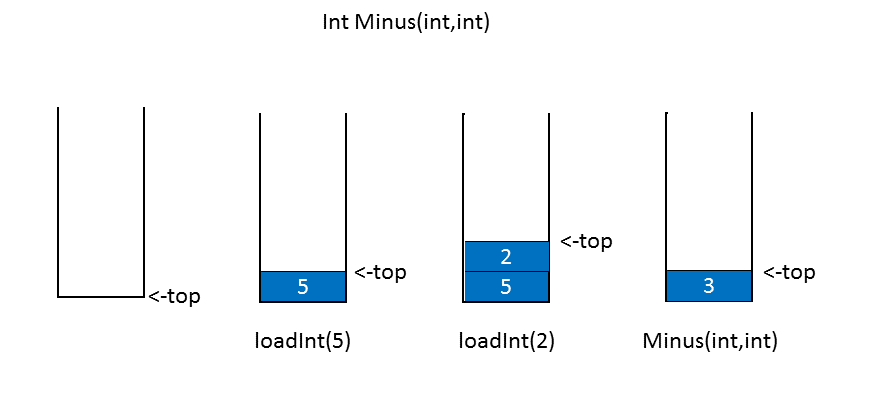
\includegraphics[scale=0.5]{images/BeispielStack.png}
\caption{Beispiel einer Minus Operation mit den Parametern (5,2)}
\label{example_stack}
\end{figure}
Eine Instruktion im MSIL Code setzt sich jeweils aus einem OpCode und einem Operand zusammen.
\begin{lstlisting}
ldsflda    class TestProgram.NewObject TestProgram.Program::_obj1
\end{lstlisting}
In diesem Beispiel eines IL Code ist "ldsflda" der OpCode und "class TestProgram.NewObject TestProgram.Program::\_obj1" der Operand. Der OpCode (Operation Code) identifiziert was die Operation durchführen soll. Hier "ldsflda" (Load Static Field Address). Dabei wird vom Operand definierten Static Field die Speicheradresse ausgelesen und auf den Stack gelegt. Der Operand ist daher jeweils die Ressource welche für den OpCode verwendet wird. Der Typ des Operand ist durch den OpCode definiert.\\
Um erfolgreich den Source Code für den Dynamic Parallel Checker zu instrumentieren (sh. \autoref{example_injection}), muss der Aufbau des Stacks immer sichergestellt werden. Daher müssen Werte um Sie aus dem Stack herauszulesen, immer dupliziert werden, damit das Programm erfolgreich durchgeführt werden kann.\\
\begin{figure}[H]
\centering
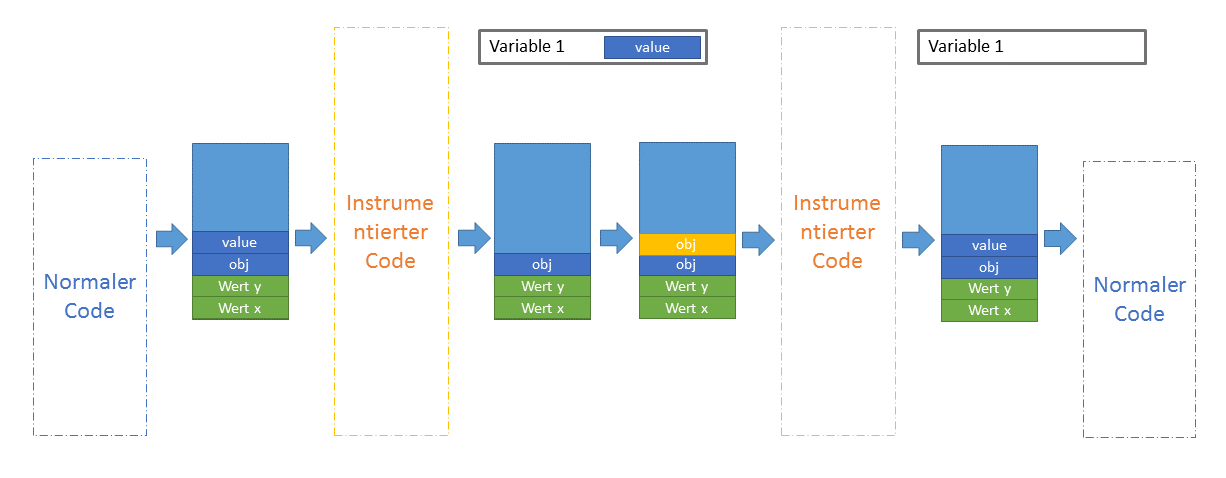
\includegraphics[scale=0.5]{images/BeispielInjection.png}
\caption{Beispiel Code Injection, Stack Verhalten}
\label{example_injection}
\end{figure}
In \autoref{example_injection} ist ein Beispiel dargestellt, wie eine Injection den Stack verwaltet und dabei die benötigte Information "obj" aus dem Stack extrahiert und den Ursprungszustand wiederherstellt. Da bei einem LIFO Stack nur auf das oberste Element zugegriffen werden kann, wird der Top-Wert "value" in eine lokale Variable gespeichert. Nach dem Abbau des duplizieren "obj" wird der Wert wieder aus der Variable auf den Stack gelegt.
\end{flushleft}
\subsection{Implementation}\label{implementation}
In diesem Kapitel wird die Implementation des Dynamic Prallel Checker genauer erklärt. Unter \ref{example} ist das Beispiel beschrieben an welchem, in den folgenden Kapitel, die Funktion des Dynamic Parallel Checkers beschrieben wird. Der Dynamic Parallel Checker wurde mit C\#.Net entwickelt.
\newpage
\subsubsection{Beispiel}\label{example}
\begin{flushleft}
Der Vektor Clock Algorithmus wird in diesem Kapitel mit Hilfe von folgendem Pseudo-Code Beispiel genauer erläutert.\\
\begin{figure}[H]
\begin{singlespace}
\begin{lstlisting}[basicstyle=\small]
//... Deklaration a,b,locka,lockb...

Thread.Start(() =>		// start thread2 (T2)
{
	lock(lockb) {
		b = 3;
	}
	b = 4;
	lock(locka) {
		Console.WriteLine(a);
	}
});
Thread.Start(() =>		// start thread3 (T3)
{
	lock(locka) {
		a = 2;
	}
	b = 5;
	lock(lockb) {
		Console.WriteLine(b);
	}
})
lock(locka) {
	a = 3;
}
lock(lockb) {
	b = 6;
}
Console.WriteLine(a);
\end{lstlisting}
\end{singlespace}
\caption{Beispiel für die Erklärung des Algorithmus}\label{basic_example}
\end{figure}
Da der Code in \autoref{basic_example} asynchron durchgeführt wird, werden die 3 enstehenden Thread parallel ausgeführt. \autoref{basic_example_parallel} zeigt was die einzelnen Threads parallel durchführen. "w( ), r( )" stehen für Write und Read Vorgänge des Threads. Der Buchstabe in der Klammer für die Ressource.
\begin{figure}[H]
\centering
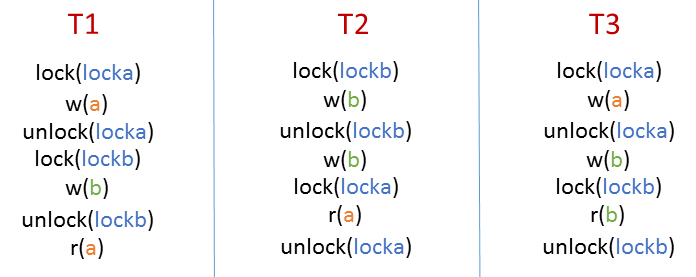
\includegraphics[scale=0.5]{images/VectorCheckingAlgorithm.png}
\caption{Darstellung der parallelen Vorgänge von \autoref{basic_example}}
\label{basic_example_parallel}
\end{figure}
\end{flushleft}
\newpage
\subsubsection{Instrumentation}
\begin{flushleft}
Für die Durchführung des Vector Clock Algorithmus (sh. Kapitel \ref{vector_algorithm}) ist es wichtig die Informationen über Lese- / Schreibzugriffe sowie Locks und Thread.Starts zu erhalten. Dazu muss der bestehende IL Code angepasst (instrumentiert) werden, damit er diese Informationen preisgibt. Dazu wird der Code analysiert und an Stellen mit wichtigen Zugriffen um Code erweitert. Wie in Kapitel \ref{chapter_IL} bereits beschrieben muss dabei der korrekte Aufbau des Stack jederzeit sichergestellt werden. Für die Instrumentation des Codes wird die Library Mono.Cecil aus dem Mono Projekt verwendet. Die Library erlaubt es den IL Code zu lesen und zu bearbeiten. 
\begin{figure}[H]
\centering
\begin{lstlisting}[language=CIL,backgroundcolor=\color{backcolor}]
IL_001a:  box        [mscorlib]System.Int32
IL_001f:  stsfld     object TestProgram.Program::_a
\end{lstlisting}
\caption{Beispiel ohne Instrumentation}\label{example_codeWithoutInstrum}
\end{figure}
\autoref{example_codeWithoutInstrum} zeigt ein Beispiel, eines typischen Schreibzugriff im MS IL. Der Befehl "box" führt ein Boxing eines Integers durch. Dabei wird der Integerwert von einem Valuetype zu einem Referenztyp umgebaut. Auf dem Stack liegt nach dem Boxing die Adresse des Integer-Werts. Diese Adresse wird dann verwendet um den Wert in die Variable "\_a" mit dem Befehl "stsfld"(Store Static Field) zu speichern.\\
\begin{figure}[H]
\centering
\begin{lstlisting}[language=CIL,backgroundcolor=\color{backcolor}]
IL_001a:  box        [mscorlib]System.Int32
//----------Instrumented Code...----------------
IL_001f:  ldsflda    object TestProgram.Program::_a
IL_0024:  ldc.i4.s   31
IL_0026:  ldstr      "System.Void TestProgram.Program::Test()"
IL_002b:  call       void [DPCLibrary]DPCLibrary.DpcLibrary::
                                 WriteAccess(int32,int32,string)
//----------...End Instrumentation--------------
IL_0030:  stsfld     object TestProgram.Program::_a
\end{lstlisting}
\caption{Instrumentierter IL Code}\label{example_instrumentedCode}
\end{figure}
\autoref{example_instrumentedCode} zeigt den Code nach dem der Dynamic Parallel Checker diesen instrumentiert hat. Wie in \autoref{example_codeWithoutInstrum}, startet der Code mit "box" und endet mit "stsfld". Dazwischen wurde der Code um den Dynamic Parallel Checker erweitert. Um zu wissen auf welche Variable der Schreibzugriff durchgeführt wird, wird mit "ldsflda" (Load static Field Address) die Adresse der Resource ausgelesen und auf den Stack gelegt. Danach wird die Zeilennummer des Schreibzugriff auf den Stack gelegt (Man beachte: Die Zeilennummer zeigt die Zeile vor der Instrumentation) um bei einem Fehler aufzuzeigen, welche Code Zeilen diesen verursacht haben. Daher wird auch als nächstes der Methodennamen als String auf den Stack gelegt. Als letzte instrumentierte Zeile werden dann die Informationen an den Dynamic Parallel Checker übergeben. Dies wird mit der Methode "WriteAccess(int32,int32,string)" durchgeführt. Nach dem Instrumentierten Code hat der Stack wieder den gleichen Zustand wie nach dem "Box" Befehl in \autoref{example_codeWithoutInstrum}.
\end{flushleft}
\subsubsection{Vector Clock pro Thread}
\begin{flushleft}
Die Vector Clock eignet sich optimal for die History des Dynamic Parallel Checkers. Jeder Thread erhält seine eigene Vektor Clock, in der er die Zeitstempel der anderen Threads mitführt. Es wird nicht der aktuelle Zeitstempel mitgeführt, sondern der Zeitstempel der bei der letzten direkten oder indirekten Synchronisation mit diesem Thread von diesem Thread mitgeliefert wurde. Bei einem Synchronisationspunkt wird die Vector Clock mit der Vector Clock aus der Lock-History synchronisiert. (sh. \ref{lock_history}) Die Reihenfolge der Synchronisation ist jedoch nicht deterministisch und hängt vom Scheduler ab.\\
Unser Algorithmus verwendet die Vector Clock des aktuellen Threads um diese mit den Vector Clocks der History der anderen Threads zu vergleichen, um herauszufinden welche Zugriffe neben läufig zu dem aktuellen Zugriff stattgefunden haben. Daher ist es sehr wichtig, dass jeder Thread seine eigene Vector Clock hat.
\end{flushleft}
\subsubsection{Lock-History}\label{lock_history}
\begin{flushleft}
Während der kompletten Überwachung wird eine Lock-History (\autoref{example_lockHistory}) geführt. Diese beinhaltet die Information welcher Thread auf welche Ressource zu welcher Zeit (Vector Clock) einen Lock durchgeführt hat. Diese Information wird benötigt um z.B. eine Synchronisation zwischen dem Thread, der den letzten Unlock auf eine Ressource durchgeführt hat, mit dem aktuellen Thread, der nun einen Lock auf die selbe Ressource durchführen möchte, vorzunehmen. Bei jedem Unlock wird ein neuer Lock-History Eintrag erstellt, falls noch keiner vorhanden ist. Sollte jedoch bereits einer vorhanden sein, wird dieser einfach überschrieben.\\
\end{flushleft}
\begin{figure}[H]
\begin{center}
\textbf{\textit{Lock-History:}}\\[0.5cm]
\begin{tabular}{ c c c }
  Vektor & Ressource & ThreadNr \\\hline
  (2,1,0) & locka & 1 \\
  (0,1,0) & lockb & 2 \\\hline\\
\end{tabular}
\caption{Beispiel Lock-History}\label{example_lockHistory}
\end{center}
\end{figure}
\textbf{Synchronisation der Vector Clock}
\begin{flushleft}
Wenn z.B. im Beispielprogramm (\autoref{basic_example}) Thread1 (T1) vor Thread3 (T3) in den Lock(a) Bereich kommt, schreibt er beim Verlassen des gesicherten Bereichs einen Eintrag in die Lock-History. Wenn nun T3 den Lock(a) beziehen möchte, prüft der Algorithmus zuerst, ob ein Eintrag in der Lock-History vorhanden ist. Ist die der Fall, wird die eigene Vector Cock (a3, b3, c3) mit der Vector Clock des History Eintrags (a1, b1, c1) synchronisiert. (\autoref{example_vectorClockSync})\\
\newpage
Vorgehensweise bei der Synchronisation:
\begin{itemize}
\item Bei jeder ThreadId oder TaskId, die in den beiden Vector Clock vorkommt, wird der grössere Wert aus beiden Vector Clocks verwendet. z.B. MAX(a1, a2)
\item Die synchronisierende Vector Clock inkrementiert den Wert der eigenen ThreadId oder TaskId. z.B. MAX(c1, c3) + 1
\end{itemize}
\begin{figure}[H]
\[
	T1 = \begin{pmatrix}
		T1 & 2\\
		T2 & 1\\
	\end{pmatrix},
	T3_{alt} = \begin{pmatrix}
		T2 & 2\\
		T3 & 3\\
	\end{pmatrix} =>
	T3_{neu} = \begin{pmatrix}
		T1 & MAX(2, 0) = 2\\
		T2 & MAX(1, 2) = 2\\
		T3 & MAX(0, 3) + 1 = 4\\
	\end{pmatrix}
\]
\caption{Beispiel Vector Clock Synchronisation}\label{example_vectorClockSync}
\end{figure}
Somit stehen alle Zugriffe, von vor der Synchronisation von Thread1, in der Happened-Before Beziehung mit allen Zugriffen von Thread3 nach der Synchronisation. Somit können diese Zugriffe keine Race Condition darstellen.
\end{flushleft}
\subsubsection{Vector Clock Algorithmus}\label{vector_algorithm}
\begin{flushleft}
Mit Hilfe der Instrumentierung wird bei jedem Auftreten eines Ereignisses (Lese- oder Schreibzugriff, Lock oder Unlock auf Ressource, Start eines Threads usw.) unsere Dynamic Parallel Checker Library aufgerufen und anschliessend unser Algorithmus durchlaufen.\\[0.3cm]
Handelt es sich bei dem Ereignis im einen Lock auf eine Ressource, wird das Ablaufdiagramm in \autoref{algo_lock} durchlaufen. Zuerst wird überprüft, ob in der Lock-History bereits ein Eintrag vorhanden ist, der auf die gleiche Ressource lautet. Ist dies der Fall, findet eine Synchronisation zwischen der Vector Clock des aktuellen Threads und der Vector Clock des Eintrags in der Lock-History statt. Die Synchronisation ist in \ref{lock_history} beschrieben.\\
\begin{figure}[H]
\centering
	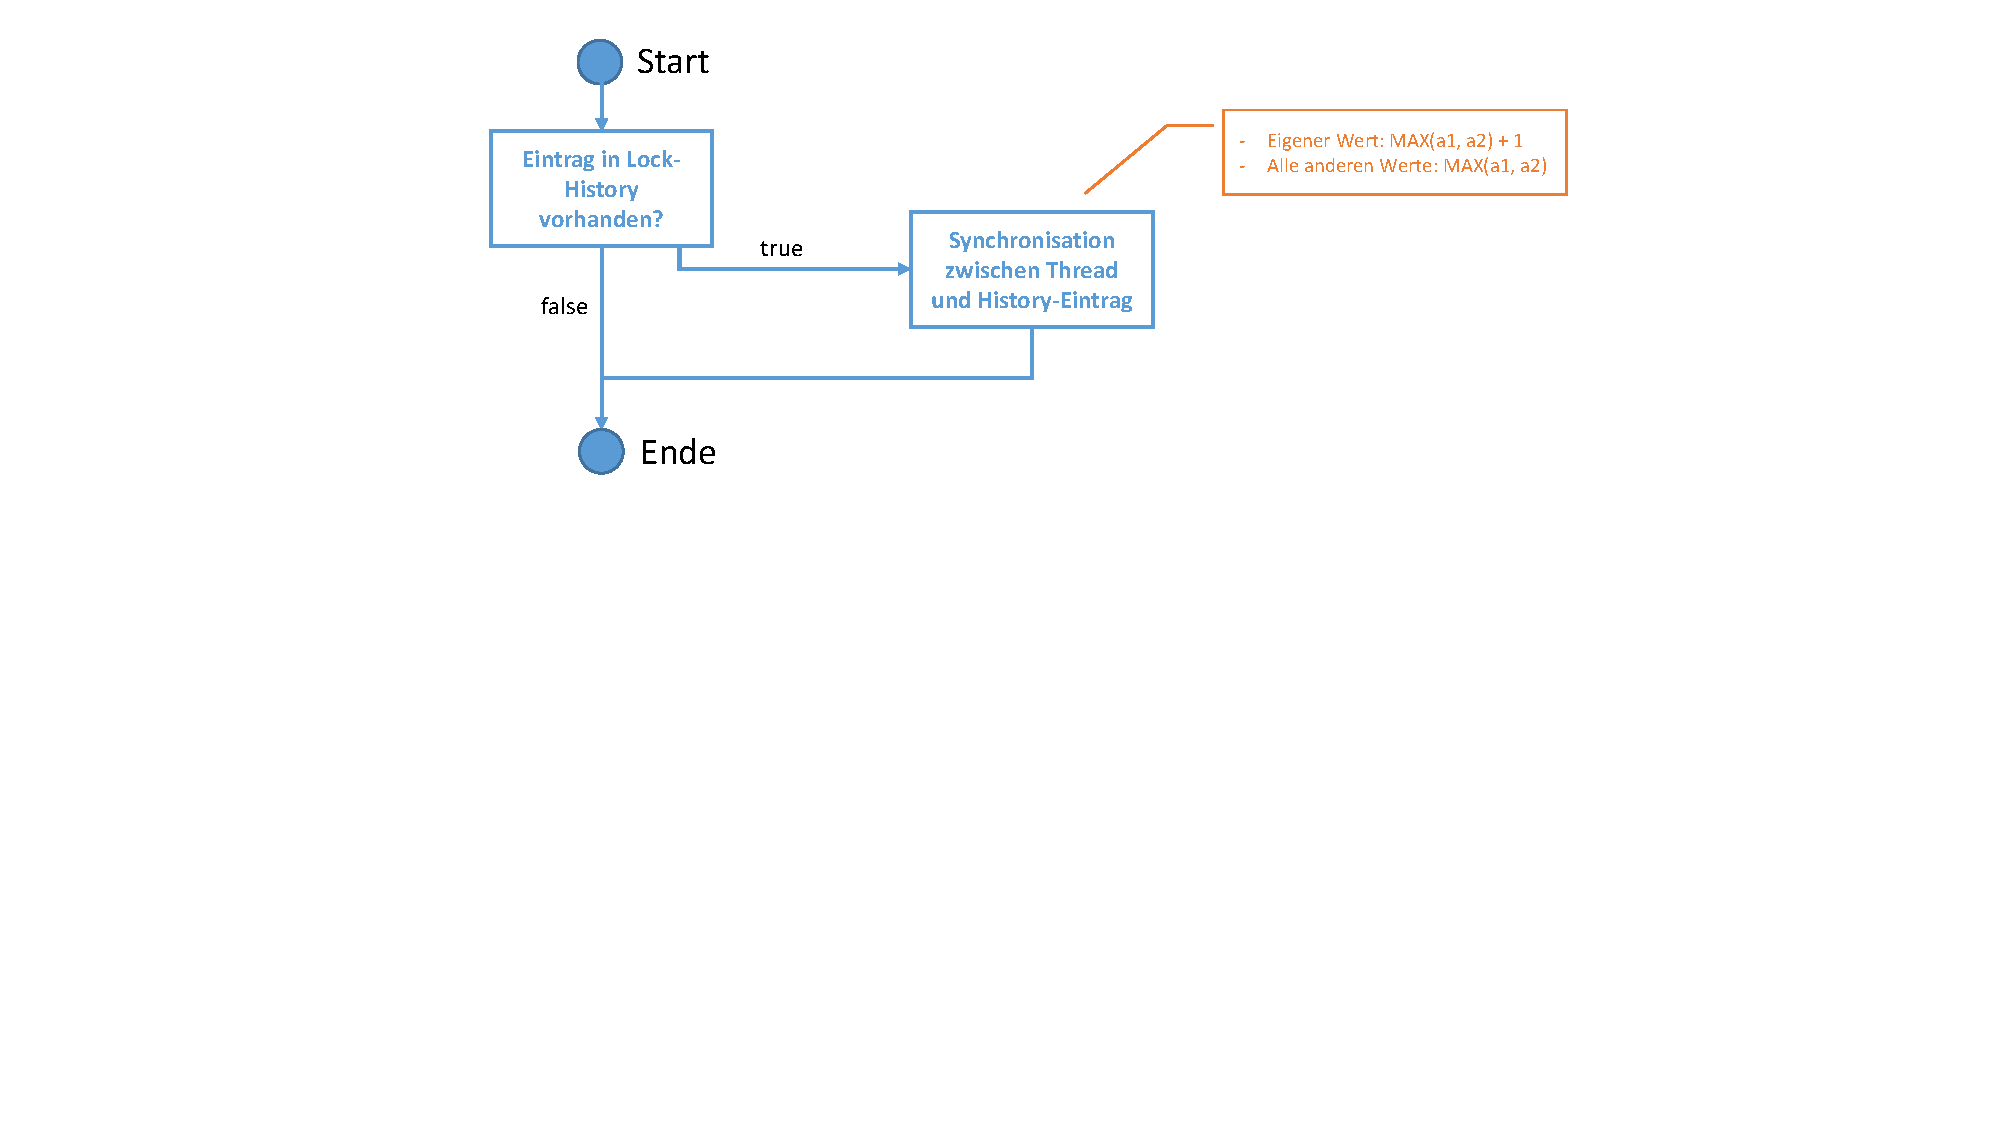
\includegraphics[width=14cm,height=5.5cm,trim=70mm 110mm 70mm 5mm, clip]{images/Lock.pdf}
\caption{Algorithmus - Lock}\label{algo_lock}
\end{figure}
Handelt es sich bei dem Ereignis um einen Unlock auf eine Ressource, wird das Ablaufdiagramm in \autoref{algo_unlock} durchlaufen. Es wird sichergestellt, dass die aktuelle Vector Clock zu der Ressource in die Lock-History geschrieben wird. Dabei wird überprüft, ob bereits ein Eintrag zu dieser Ressource in der Lock-History vorhanden ist. Wenn ja, wird dieser mit der neuen Zeit und der ThreadId oder TaskId überschrieben. Falls kein Eintrag vorhanden ist wird ein Neuer erstellt. Zudem wird der eigene Wert in der Vector Clock des aktuellen Threads oder Tasks inkrementiert. Dies dient dazu, dass beim nächsten Auftreten eines Locks auf dieselbe Ressource, nach der Synchronisation, die Happened-Before Beziehung gilt. \\
\begin{figure}[H]
\centering
	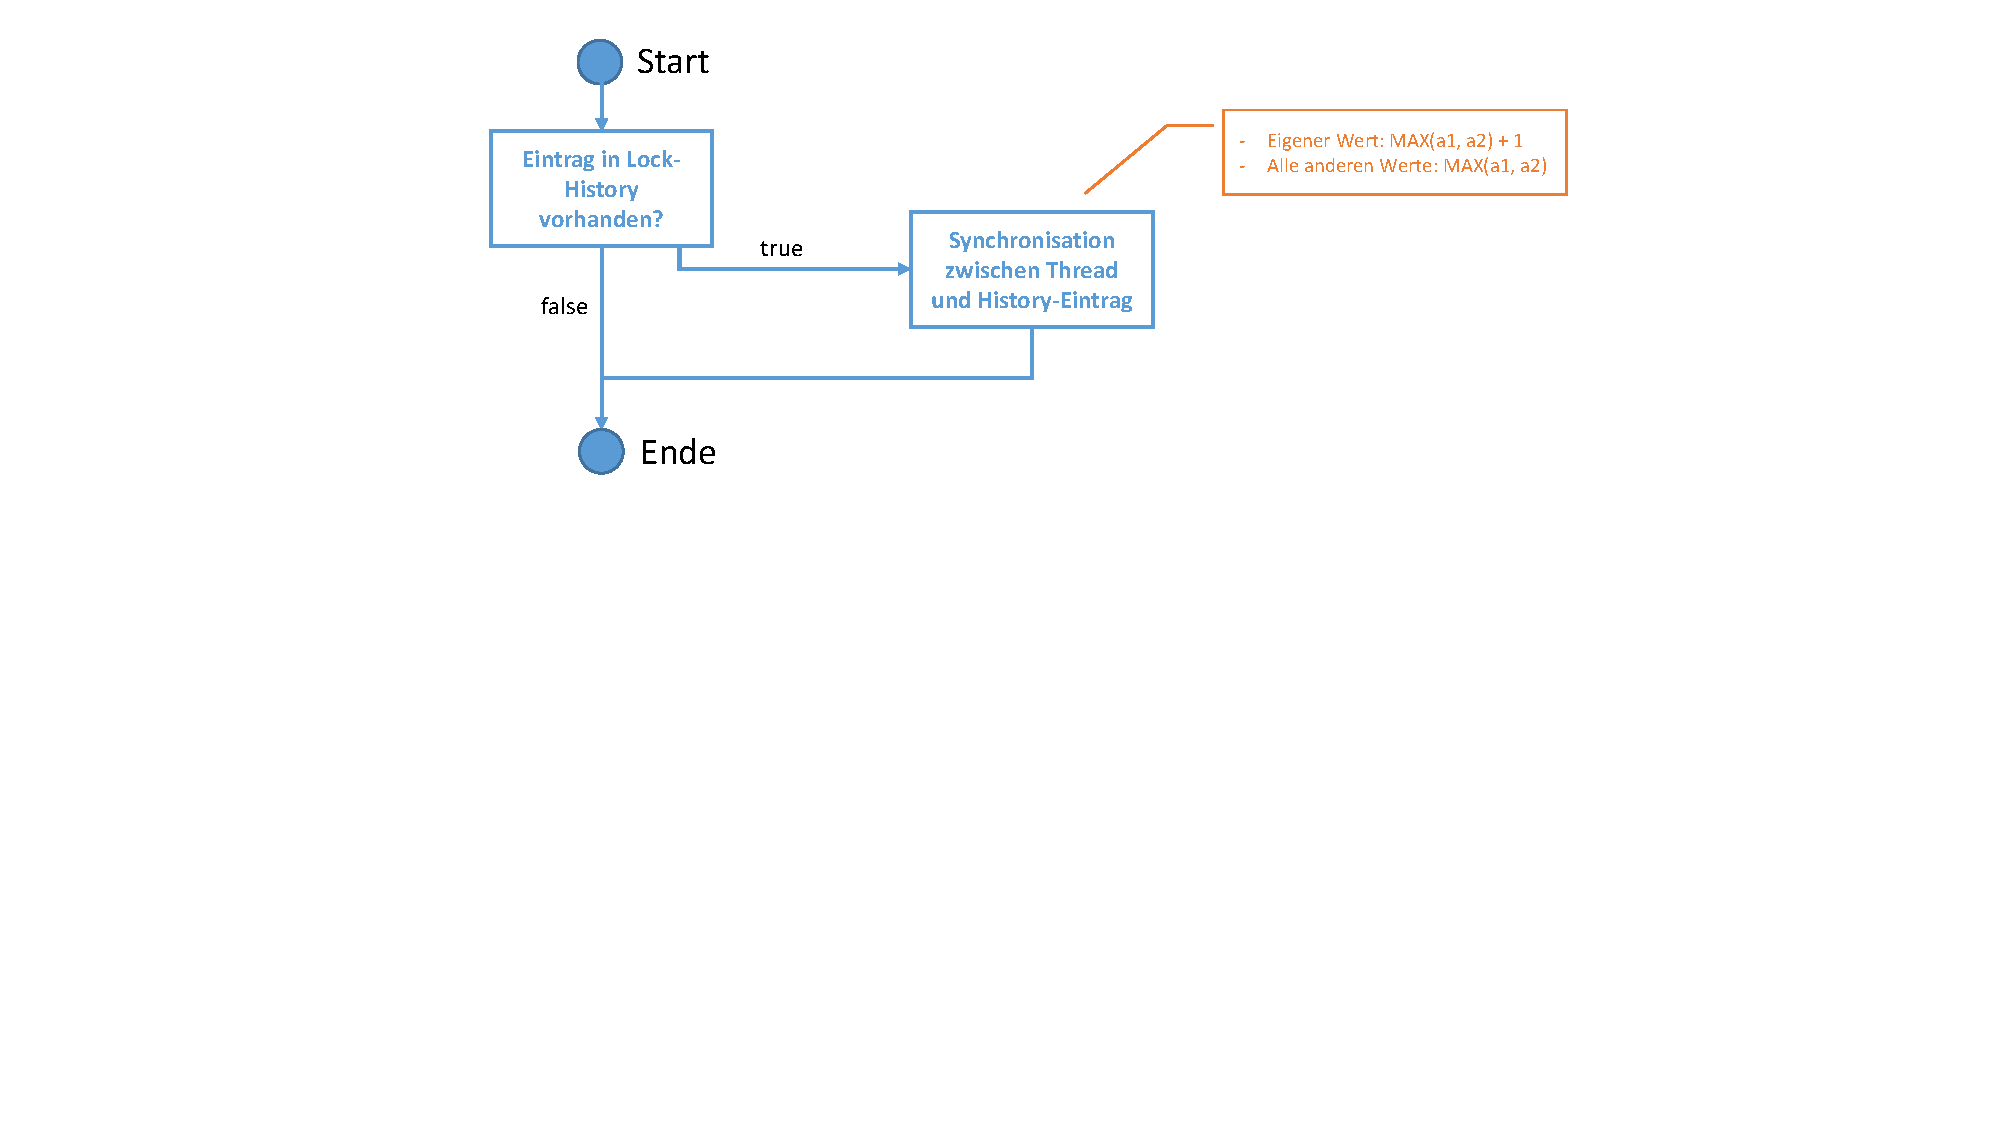
\includegraphics[width=12cm,height=5.5cm,trim=70mm 106mm 100mm 8mm, clip]{images/Unlock.pdf}
\caption{Algorithmus - Unlock}\label{algo_unlock}
\end{figure}
Handelt es sich bei dem Ereignis um einen Lese- oder Schreibzugriff auf eine Ressource, wird das Ablaufdiagramm in \autoref{algo_readwrite} durchlaufen. Zuerst wird das Ereignis in die Program-History des aktuellen Threads oder Tasks abgelegt. Sollte während der selben Vector Clock Zeit, im aktuellen Thread, bereits ein Zugriff auf diese Ressource stattgefunden haben, wird der Zugriffstyp (Read oder Write) aktualisiert. Solange nur Lesezugriffe stattgefunden haben ist der Zugriffstyp immer "Read". Sobald jedoch ein Schreibzugriff stattgefunden hat wird dieser Typ auf "Write" geändert und wird nie mehr den Type "Read" erhalten. Dadurch wurde die Datenstruktur optimiert.\\
Anschliessend wird das aktuelle Ereignis auf Race Conditions geprüft. Dafür benötigt unser Algorithmus alle Zugriffe, von den anderen Threads oder Tasks, die neben läufig zu dem aktuellen Zugriff aufgetreten sind. Dies kann mit Hilfe der Happened-Before Beziehung überprüft werden. In einem dynamischen Checker hat das Scheduling einen grossen Einfluss auf die Reihenfolge der einzelnen Zugriffe und kann dadurch die Happened-Before Beziehungen zwischen zwei Zugriffen ändern.\\
Hat einer dieser neben läufigen Zugriffe auf die selbe Ressource zugegriffen, wird überprüft ob es sich dabei um eine Race Condition handelt. Mehr Informationen zu Race Conditions in Kapitel \ref{race_conditons}. Sollte eine Race Condition erkannt werden, wird diese mit Hilfe des Logging Frameworks NLog an die WPF Applikation gemeldet und dem Benutzer angezeigt.
\begin{figure}[H]
\centering
	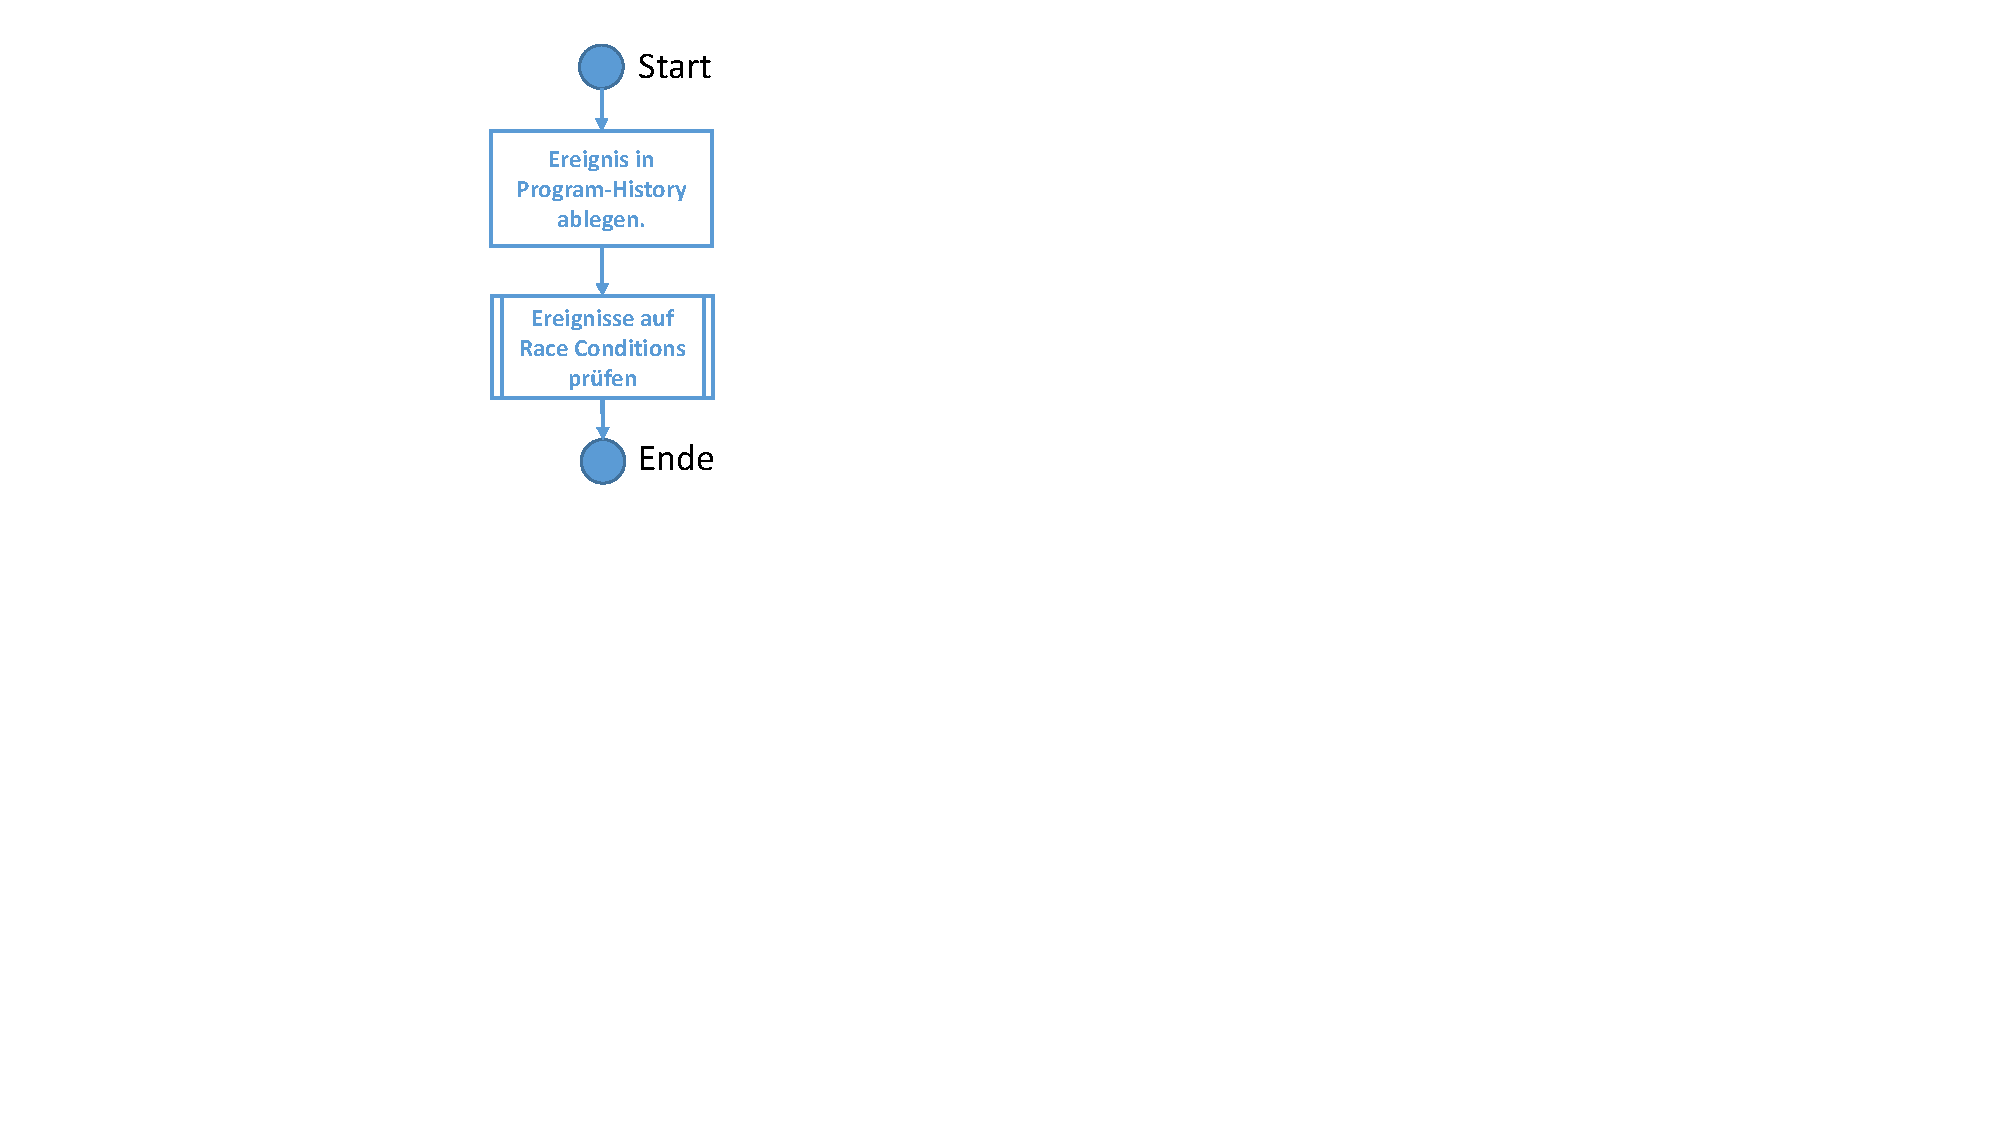
\includegraphics[width=5cm,height=5.5cm,trim=70mm 108mm 200mm 7mm, clip]{images/ReadWrite.pdf}
\caption{Algorithmus - Read/Write}\label{algo_readwrite}
\end{figure}
\end{flushleft}
\textbf{Algorithmus Beispiel}
\begin{flushleft}
In diesem Kapitel wird der Algorithmus auf das Beispielprogramm  in \autoref{basic_example} angewendet. Dabei ist zu beachten, dass dieses Beispiel lediglich eine mögliche Ablaufsequenz aufzeigt. Änderst sich das Scheduling, ändert sich auch das komplette Verhalten des Algorithmus.\\
\begin{itemize}
\item \textit{Alle Threads werden gestartet. Jede Instanz eines Threads oder Tasks instanziiert eine neue Vector Clock. Die Lock-History sowie die Programm-History ist noch leer.}\\[0.3cm]
\begin{tabular}{ >{\small}c >{\small}c >{\small}c }
  	Vektor & Ressource & ThreadNr \\\hline
  	  &   &   \\\hline
\end{tabular}\hspace*{0.5cm}
\begin{tabular}{ >{\small}c >{\small}c >{\small}c >{\small}c }
  	ThreadNr & Ressource & Vektor & ZugriffsTyp \\\hline
  	  &   &   &   \\\hline
\end{tabular}
\[
	T1 = \begin{pmatrix}
		T1 & 1\\
	\end{pmatrix}
	, T2 = \begin{pmatrix}
		T2 & 1\\
	\end{pmatrix}
	, T3 = \begin{pmatrix}
		T3 & 1\\
	\end{pmatrix}
\]
\item \textit{lock(lockb), w(b), unlock(lockb) von Thread2}\\[0.3cm]
\begin{tabular}{ >{\small}c >{\small}c >{\small}c }
  	Vektor & Ressource & ThreadNr \\\hline
  	(0,1,0) & lockb & 2 \\\hline
\end{tabular}\hspace*{0.5cm}
\begin{tabular}{ >{\small}c >{\small}c >{\small}c >{\small}c }
  	ThreadNr & Ressource & Vektor & ZugriffsTyp \\\hline
  	2 & b & (0,1,0) & write \\\hline
\end{tabular}
\[
	T1 = \begin{pmatrix}
		T1 & 1\\
	\end{pmatrix}
	, T2 = \begin{pmatrix}
		T2 & 2\\
	\end{pmatrix}
	, T3 = \begin{pmatrix}
		T3 & 1\\
	\end{pmatrix}
\]
\item \textit{lock(locka), w(a), unlock(locka) von Thread1}\\[0.3cm]
\begin{tabular}{ >{\small}c >{\small}c >{\small}c }
  	Vektor & Ressource & ThreadNr \\\hline
  	(1,0,0) & locka & 1 \\
  	(0,1,0) & lockb & 2 \\\hline
\end{tabular}\hspace*{0.5cm}
\begin{tabular}{ >{\small}c >{\small}c >{\small}c >{\small}c }
  	ThreadNr & Ressource & Vektor & ZugriffsTyp \\\hline
  	2 & b & (0,1,0) & write \\
  	1 & a & (1,0,0) & write \\\hline
\end{tabular}
\[
	T1 = \begin{pmatrix}
		T1 & 2\\
	\end{pmatrix}
	, T2 = \begin{pmatrix}
		T2 & 2\\
	\end{pmatrix}
	, T3 = \begin{pmatrix}
		T3 & 1\\
	\end{pmatrix}
\]\newpage
\item \textit{lock(locka), w(a), unlock(locka) von Thread3. Keine Race Condition, weil Happened Before Beziehung zwischen beiden Schreibzugriffen auf Ressource a.}\\[0.3cm]
\begin{tabular}{ >{\small}c >{\small}c >{\small}c }
  	Vektor & Ressource & ThreadNr \\\hline
  	(1,0,2) & locka & 3 \\
  	(0,1,0) & lockb & 2 \\\hline
\end{tabular}\hspace*{0.5cm}
\begin{tabular}{ >{\small}c >{\small}c >{\small}c >{\small}c }
  	ThreadNr & Ressource & Vektor & ZugriffsTyp \\\hline
  	2 & b & (0,1,0) & write \\
  	\color{ForestGreen}1 & \color{ForestGreen}a & \color{ForestGreen}(1,0,0) & \color{ForestGreen}write \\
  	\color{ForestGreen}3 & \color{ForestGreen}a & \color{ForestGreen}(1,0,2) & \color{ForestGreen}write \\\hline
\end{tabular}
\[
	T1 = \begin{pmatrix}
		T1 & 2\\
	\end{pmatrix}
	, T2 = \begin{pmatrix}
		T2 & 2\\
	\end{pmatrix}
	, T3 = \begin{pmatrix}
		T1 & 1\\		
		T3 & 3\\
	\end{pmatrix}
\]
\item \textit{w(b) von Thread2}\\[0.3cm]
\begin{tabular}{ >{\small}c >{\small}c >{\small}c }
  	Vektor & Ressource & ThreadNr \\\hline
  	(1,0,2) & locka & 3 \\
  	(0,1,0) & lockb & 2 \\\hline
\end{tabular}\hspace*{0.5cm}
\begin{tabular}{ >{\small}c >{\small}c >{\small}c >{\small}c }
  	ThreadNr & Ressource & Vektor & ZugriffsTyp \\\hline
  	2 & b & (0,1,0) & write \\
  	1 & a & (1,0,0) & write \\
  	3 & a & (1,0,2) & write \\
  	2 & b & (0,2,0) & write \\\hline
\end{tabular}
\[
	T1 = \begin{pmatrix}
		T1 & 2\\
	\end{pmatrix}
	, T2 = \begin{pmatrix}
		T2 & 2\\
	\end{pmatrix}
	, T3 = \begin{pmatrix}
		T1 & 1\\		
		T3 & 3\\
	\end{pmatrix}
\]
\item \textit{w(b) von Thread3. Eine Race Condition ist aufgetreten.}\\[0.3cm]
\begin{tabular}{ >{\small}c >{\small}c >{\small}c }
  	Vektor & Ressource & ThreadNr \\\hline
  	(1,0,2) & locka & 3 \\
  	(0,1,0) & lockb & 2 \\\hline
\end{tabular}\hspace*{0.5cm}
\begin{tabular}{ >{\small}c >{\small}c >{\small}c >{\small}c }
  	ThreadNr & Ressource & Vektor & ZugriffsTyp \\\hline
  	2 & b & (0,1,0) & write \\
  	1 & a & (1,0,0) & write \\
  	3 & a & (1,0,2) & write \\
  	\color{red}2 & \color{red}b & \color{red}(0,2,0) & \color{red}write\\
  	\color{red}3 & \color{red}b & \color{red}(1,0,3) & \color{red}write \\\hline
\end{tabular}
\[
	T1 = \begin{pmatrix}
		T1 & 2\\
	\end{pmatrix}
	, T2 = \begin{pmatrix}
		T2 & 2\\
	\end{pmatrix}
	, T3 = \begin{pmatrix}
		T1 & 1\\		
		T3 & 3\\
	\end{pmatrix}
\]
\item \textit{lock(lockb), w(b), unlock(lockb) von Thread1. Zwei Race Conditions sind aufgetreten.}\\[0.3cm]
\begin{tabular}{ >{\small}c >{\small}c >{\small}c }
  	Vektor & Ressource & ThreadNr \\\hline
  	(1,0,2) & locka & 3 \\
  	(3,1,0) & lockb & 1 \\\hline
\end{tabular}\hspace*{0.5cm}
\begin{tabular}{ >{\small}c >{\small}c >{\small}c >{\small}c }
  	ThreadNr & Ressource & Vektor & ZugriffsTyp \\\hline
  	2 & b & (0,1,0) & write \\
  	1 & a & (1,0,0) & write \\
  	3 & a & (1,0,2) & write \\
  	\color{red}2 & \color{red}b & \color{red}(0,2,0) & \color{red}write\\
  	\color{red}3 & \color{red}b & \color{red}(1,0,3) & \color{red}write \\
  	\color{red}1 & \color{red}b & \color{red}(3,1,0) & \color{red}write \\\hline
\end{tabular}
\[
	T1 = \begin{pmatrix}
		T1 & 4\\
		T2 & 1\\
	\end{pmatrix}
	, T2 = \begin{pmatrix}
		T2 & 2\\
	\end{pmatrix}
	, T3 = \begin{pmatrix}
		T1 & 1\\		
		T3 & 3\\
	\end{pmatrix}
\]
\item \textit{lock(locka), r(a), unlock(locka) von Thread2. Eine Race Condition ist aufgetreten.}\\[0.2cm]
\begin{tabular}{ >{\small}c >{\small}c >{\small}c }
  	Vektor & Ressource & ThreadNr \\\hline
  	(1,3,2) & locka & 2 \\
  	(3,1,0) & lockb & 1 \\\hline
\end{tabular}\hspace*{0.5cm}
\begin{tabular}{ >{\small}c >{\small}c >{\small}c >{\small}c }
  	ThreadNr & Ressource & Vektor & ZugriffsTyp \\\hline
  	2 & b & (0,1,0) & write \\
  	1 & a & (1,0,0) & write \\
  	\color{red}3 & \color{red}a & \color{red}(1,0,2) & \color{red}write \\
  	2 & b & (0,2,0) & write\\
  	3 & b & (1,0,3) & write \\
  	1 & b & (3,1,0) & write \\
  	\color{red}2 & \color{red}a & \color{red}(1,3,2) & \color{red}read \\\hline
\end{tabular}
\[
	T1 = \begin{pmatrix}
		T1 & 4\\
		T2 & 1\\
	\end{pmatrix}
	, T2 = \begin{pmatrix}
		T1 & 1\\		
		T2 & 4\\
		T3 & 2\\
	\end{pmatrix}
	, T3 = \begin{pmatrix}
		T1 & 1\\		
		T3 & 3\\
	\end{pmatrix}
\]
\item \textit{lock(lockb), r(b), unlock(lockb) von Thread3. Eine Race Condition ist aufgetreten.}\\[0.2cm]
\begin{tabular}{ >{\small}c >{\small}c >{\small}c }
  	Vektor & Ressource & ThreadNr \\\hline
  	(1,3,2) & locka & 2 \\
  	(3,1,4) & lockb & 3 \\\hline
\end{tabular}\hspace*{0.5cm}
\begin{tabular}{ >{\small}c >{\small}c >{\small}c >{\small}c }
  	ThreadNr & Ressource & Vektor & ZugriffsTyp \\\hline
  	2 & b & (0,1,0) & write \\
  	1 & a & (1,0,0) & write \\
  	3 & a & (1,0,2) & write \\
  	\color{red}2 & \color{red}b & \color{red}(0,2,0) & \color{red}write\\
  	3 & b & (1,0,3) & write \\
  	1 & b & (3,1,0) & write \\
  	2 & a & (1,3,2) & read \\
  	\color{red}3 & \color{red}b & \color{red}(3,1,4) & \color{red}read \\\hline
\end{tabular}
\[
	T1 = \begin{pmatrix}
		T1 & 4\\
		T2 & 1\\
	\end{pmatrix}
	, T2 = \begin{pmatrix}
		T1 & 1\\		
		T2 & 4\\
		T3 & 2\\
	\end{pmatrix}
	, T3 = \begin{pmatrix}
		T1 & 3\\
		T2 & 1\\		
		T3 & 5\\
	\end{pmatrix}
\]
\item \textit{r(a) von Thread1. Eine Race Condition ist aufgetreten.}\\[0.2cm]
\begin{tabular}{ >{\small}c >{\small}c >{\small}c }
  	Vektor & Ressource & ThreadNr \\\hline
  	(1,3,2) & locka & 2 \\
  	(3,1,4) & lockb & 3 \\\hline
\end{tabular}\hspace*{0.5cm}
\begin{tabular}{ >{\small}c >{\small}c >{\small}c >{\small}c }
  	ThreadNr & Ressource & Vektor & ZugriffsTyp \\\hline
  	2 & b & (0,1,0) & write \\
  	1 & a & (1,0,0) & write \\
  	\color{red}3 & \color{red}a & \color{red}(1,0,2) & \color{red}write \\
  	... & ... & ... & ... \\
  	2 & a & (1,3,2) & read \\
  	3 & b & (3,1,4) & read \\
  	\color{red}1 & \color{red}a & \color{red}(4,1,0) & \color{red}read \\\hline
\end{tabular}
\[
	T1 = \begin{pmatrix}
		T1 & 4\\
		T2 & 1\\
	\end{pmatrix}
	, T2 = \begin{pmatrix}
		T1 & 1\\		
		T2 & 4\\
		T3 & 2\\
	\end{pmatrix}
	, T3 = \begin{pmatrix}
		T1 & 3\\
		T2 & 1\\		
		T3 & 5\\
	\end{pmatrix}
\]
\end{itemize}
\end{flushleft}
\newpage
\section{Schlussfolgerungen}
TODO\\
\subsection{Performance}
\subsection{Technische Findings}
\subsubsection{Task/Threads}
\begin{flushleft}
Das .Net Framework von Microsoft kennt zwei asynchrone Operationstypen. Task oder Threads. Der Unterschied dieser zwei Typen liegt auf der Ausführungsumgebung. Threads werden direkt gestartet und vom Prozessor parallel verarbeitet. Task wurden zusammen mit der Task Parallel Library eingeführt. Dieser Typ wird nicht direkt ausgeführt, sondern in eine Queue geladen und dann von Worker Threads berechnet. Die Worker Threads werden vom .Net Framework automatisch gestartet. Die Anzahl wird durch die Laufzeitumgebung bestimmt, z.B. wie viele Kernen der Prozessor hat. Der Vorteil dieser Methode gegenüber der Threads ist es, das die Belastung auf den Arbeitsspeicher und Prozessor bei vielen parallelen Vorgängen optimiert und gesenkt wird. Der Nachteil ist, das es schneller zu Deadlocks kommen kann, wenn die Threads untereinander abhängig sind.\\
Für die Entwicklung des Dynamic Parallel Checker ist der Unterschied zwischen Task und Threads dahingehend wichtig, da die ID des Threads bei Tasks der ID des Worker Thread entspricht. Um den Detailgrad der Erkennung zu erhöhen, wurde bei Tasks die Task ID und nicht die Thread ID für die Erkennung verwendet.
\end{flushleft}
\subsubsection{Garbage Collector}
\begin{flushleft}
Der Garbage Colletor (GC) verwaltet die Belegung und Freigabe von Arbeitsspeicher einer Anwendung. Bei der Erzeugung eines Objektes, wird dem Objekt die Speicherplatzadresse auf dem Heap zugewiesen. Da nicht unendlich Arbeitsspeicher vorhanden ist, greift der GC ein, und reorganisiert die Speicherplatzbelegung. Dabei kann es vorkommen, dass bestehenden Objekten eine neue Speicherstelle und somit auch eine neue Speicheradresse zugewiesen wird. Dies kann für den Dynamic Parallel Checker ein grosses Problem darstellen.\\
Der Dynamic Parallel Checker identifiziert die Objekte, auf die ein Zugriff stattgefunden hat, mit Hilfe deren Adressen. D.h. sobald der Garbage Collector den Arbeitsspeicher reorganisiert hat, haben die selben Objekte nicht mehr die gleiche Adresse und der Dynamic Parallel Checker funktioniert dadurch nicht mehr. Es gibt keine Möglichkeit die Änderungen des GCs in Erfahrung zu bringen und dadurch die gesamte History anzupassen. Sollte der GC eine Reorganisation durchführen, meldet die Dynamic Parallel Checker Library Fehlmeldungen (False-Positives).
\end{flushleft}
\subsubsection{Short Branches}
\begin{flushleft}
Der MSIL Code verwendet für Befehle wie "try/catch/finally/if/else usw." Branches. Ein Branch ist ein Befehl im IL Code welcher eine Sprungmarke definiert. Dabei wird als Operand die Code Zeile zu welcher der Branch springen soll definiert. MSIL kennt 13 verschiedene Branches (sh. \cite{ecma} III.3.5 - III.3.18 ohne III.3.16), alle funktionieren nach dem selben Prinzip. Der Operand des Befehls beinhaltet die Code Zeile, zur welcher gesprungen werden soll.\\
Durch die Instrumentation für den Dynamic Parallel Checker verändern sich die Zeilennummern. Daher ist es wichtig, dass diese nachgeführt werden. Mono.Cecil unterstützt den Entwickler soweit, das über die direkte Referenz auf die Zielcodezeile der Wert nachgetragen wird. Jedoch besitzen alle Branches neben dem Standard OpCode, auch ein "*.s" OpCode. Zum Beispiel gibt es für "brtrue IL\_3A303", den Code "brtrue.s IL\_03", wobei "*.s" nur für Code Zeilennummern kleiner "IL\_FF" verwendet werden kann. Durch die Instrumentation des Dynamic Parallel Checkers kann dieser Wert aber überschritten werden. Mono.Cecil hat keine automatische Erkennung solcher Branch-Fehler.
\begin{figure}[H]
\centering
\begin{lstlisting}[backgroundcolor=\color{backcolor}]
method.Body.SimplifyMacros();
/*-------------Code Instrumentation--------------*/
method.Body.OptimizeMacros();
\end{lstlisting}
\caption{Branch Optimierung durch Mono.Cecil}\label{branch_optimization}
\end{figure}
Die Methode SimplifyMacros in \autoref{branch_optimization} wird dazu verwendet, das Mono.Cecil alle "brtrue.s" in "brtrue" umwandelt. Dadurch kann die Zeilennummer auf die grösse die nötig ist gesetzt werden. Der Befehl OptimizeMacros versucht dann nach der Instrumentation "brtrue" wieder auf "brtrue.s" zu wandeln. Dadurch wird der Code wieder optimiert wenn möglich.\\
Wenn der Code in Mono.Cecil eingelesen wird, werden alle Adressen in den Branches als Referenz auf die jeweilige Instanz der Ziel-Methode gehalten. Wenn die Methode gelöscht wird, ist die Referenz ungültig und Mono.Cecil zeigt auf eine Unbekannte Adresse. Dadurch wird der Code instabil. Daher sollte wenn möglich Code nicht aus der Instrumentation gelöscht werden, sondern der OpCode und Operand manuell ersetzt werden.
\end{flushleft}
\section{Backlog}
\subsection{Fehlende Synchronisationsoperationen}
\begin{flushleft}
Der Umfang dieser Arbeit beschränkte sich aus zeitlichen Gründen auf einen gewissen Umfang. Die bereits instrumentierten Synchronisationspunkte befinden sich im Anhang. (sh. \nameref{sec:instrumentierte_methoden})\\
Folgende Synchronisationspunkte könnten bei einer Weiterentwicklung dieses Projekts noch umgesetzt werden:
\begin{itemize}
\setlength\itemsep{0em}
\item Thread.Abort()
\item Thread.Interrupt()
\item Task.Result()
\item Task.WaitAll()
\item Task.WaitAny()
\item Task.ContinueWith()
\item Task.WhenAll() / Task.WhenAny()
\item Task.Delay()
\item Task.Factory.ContinueWhenAny() / Task.Factory.ContinueWhenAll()
\item Task.Factory.FromAsync()
\item async await
\item volatile Variablen
\item Semaphoren
\item Finalizer
\item Parallel.Invoke() / Parallel.For() / Parallel.ForEach()
\end{itemize}
\end{flushleft}
\subsection{Funktionsweise}
\subsubsection*{Deadlock Erkennung}
Die implementierte Funktionalität erlaubt es zur Zeit nur, Race Conditions zu erkennen. Von Vorteil wäre es, wenn zusätzlich noch Deadlocks erkannt werden. Dafür müsste aber der vorhandene Algorithmus noch erweitert werden. Vor jedem Lock auf eine Ressource müsste die Dynamic Parallel Checker Library informiert werden und eine eigene Liste geführt werden, welcher Thread welchen Lock bezogen hat. Sobald ein Thread den Lock freigibt, müsste dieser Eintrag wieder gelöscht werden. Dadurch könnte erkannt werden, dass zwei unterschiedliche Threads sich gegenseitig sperren.
\subsubsection*{Dependencies instrumentieren}
In dieser Version wird eine spezifische Applikation instrumentiert. Sollte die Anwendung noch  Abhängigkeiten zu weiteren, selbst entwickelten Libraries besitzen, werden Race Conditions, aus diesen Libraries, nicht erkannt. Dies, aufgrund der Tatsache, dass die Abhängigkeiten nicht instrumentiert werden. Diese zusätzliche Funktionalität, würde den Umfang des Überprüfungsbereichs erweitern. Dabei ist zu beachten, dass die Microsoft Core Library (mscorlib) nicht mit instrumentiert wird. Dies würde den Rahmen der Überwachung sprengen.
\subsection{Vision}
\subsubsection*{Unit Testing}
\begin{flushleft}
Um die Erkennungsrate des Algorithmus erhöhen zu können, müssen Tools mehrmals den Test durchlaufen. Daher ist eine Vision, den Algorithmus in ein Concurrent-UnitTesting Framework einzubauen. Dieses erlaubt dem Entwickler das erstellen von ConcurrentTests, welche nicht nur einen synchronen Test durchführen, sondern die Tests parallel zu einander ausführt um Race Conditions zu provozieren. Der Dynamic Parallel Checker Algortihmus überwacht die Unit Tests und meldet auftretende Race Conditions. Dadurch würden Tools vor dem Deployment und im Entwicklungszyklus jederzeit auf Race Conditions getestet, was die Entwickler sensibilisiert auf parallele Probleme und die Qualität der Software erhöht. Das Unit Testing Framework kann durch einen eigenen Scheduler in der Erkennung noch weiter verbessert werden. Durch ein gezieltes Verzahnen der Threads könnte provoziert werden, dass diese Race Conditions oder Deadlocks generieren
\end{flushleft}
\section*{Glossar}
\addcontentsline{toc}{section}{Glossar}
- Partielle Ordnung\\
- Totale Ordnung\\
- Thread\\
- Task\\
\section*{Abbildungsverzeichnis}
\addcontentsline{toc}{section}{Abbildungsverzeichnis}
\makeatletter
\@starttoc{lof}
\makeatother
\section*{Literaturverzeichnis}
\addcontentsline{toc}{section}{Literaturverzeichnis}
\newcommand\oldsection{}
\let\oldsection=\section
\renewcommand{\section}[2]{}
\begin{thebibliography}{xxxxxxxxxxxxx}
\bibitem[ECMA, 2012]{ecma}"Standard ECMA-335 Common Language Infrastructure (CLI)", \href{http://www.ecma-international.org/publications/standards/Ecma-335.htm}{http://www.ecma-international.org/publications/standards/Ecma-335.htm}, 06.2012
\bibitem[MCA, 1978]{MCA}"Time, Clocks, and the Ordering of Events in a Distributed System", \href{http://research.microsoft.com/en-us/um/people/lamport/pubs/time-clocks.pdf}{http://research.microsoft.com/en-us/um/people/lamport/pubs/time-clocks.pdf}, 07.1978
\bibitem[ACSC, 1988]{acsc}"Timestamps in Message-Passing Systems That Preserve the Partial Ordering", \href{http://zoo.cs.yale.edu/classes/cs426/2012/lab/bib/fidge88timestamps.pdf}{http://zoo.cs.yale.edu/classes/cs426/2012/lab/bib/fidge88timestamps.pdf}, 02.1988
\bibitem[MSDN, 2015]{msdn}"MSDN - Memory Management and Garbage Collection", \href{https://msdn.microsoft.com/de-de/library/0xy59wtx(v=vs.110).aspx}{https://msdn.microsoft.com/de-de/library/0xy59wtx(v=vs.110).aspx}, 08.2012
\bibitem[MONO, 2015]{monocecil}"Mono.Cecil Library",\\ \href{http://www.mono-project.com/docs/tools+libraries/libraries/Mono.Cecil/}{http://www.mono-project.com/docs/tools+libraries/libraries/Mono.Cecil/}, 12.2015
\end{thebibliography}
\let\section=\oldsection
\section*{Anhang}
\addcontentsline{toc}{section}{Anhang}
\subsection*{Persönliches Fazit}
\subsubsection*{Fabian Keller}
\subsubsection*{Dominik Heeb}
\subsection*{Liste instrumentierte mscorlib Methoden}\label{sec:instrumentierte_methoden}
Bereits instrumentierte Methoden:
\begin{itemize}
\setlength\itemsep{0em}
\item Thread.Start()
\item Thread.Join()
\item Task.Start()
\item Task.Wait()
\item Task.Run()
\item Task.Factory.StartNew()
\end{itemize}
\subsection*{Liste instrumentierte MSIL Operationen}
Bereits instrumentierte MSIL Operationen:
\begin{itemize}
\setlength\itemsep{0em}
\item ldsfld (Load static field)
\item stsfld (Store static field)
\item ldfld (Load field)
\item stfld (Store field)
\item ldelem (Load element of array)
\item stelem (Store element of array)
\item initobj (Init object)
\item call (Call method)
\item callvirt (Call virtual method)
\end{itemize}
Mehr Informationen zu den einzelnen Operation Codes: siehe \cite{ecma}.
\end{document}
